\documentclass[a4paper]{article}

\usepackage{charter}
\usepackage{amssymb, amsmath}
\DeclareMathOperator*{\argmin}{arg\,min}

\let\circledS\undefined
\usepackage[charter]{mathdesign}

\usepackage[english]{babel}
\usepackage[utf8]{inputenc}
\usepackage{amsmath}
\usepackage{mathtools}
\usepackage{caption}
\usepackage{subcaption}
\usepackage{graphicx}
\usepackage[colorinlistoftodos]{todonotes}
\usepackage{booktabs}
\usepackage{listings}
\usepackage{nopageno}

\usepackage{titlesec}
\titleformat{\section}{\Large\scshape}{\thesection}{1em}{}
\titleformat{\subsection}{\large\scshape}{\thesection}{1em}{}
\titlespacing*{\section}{0em}{1em}{0.5em}
\titlespacing*{\subsection}{0em}{1em}{0.5em}

% \usepackage[top=1in, bottom=1.25in, left=2in, right=2in]{geometry}

\usepackage{hyperref}
\newcommand{\qued}{\hfill $\blacksquare$}
\newcommand*\de{\mathop{}\!\mathrm{d}}
\newtheorem{lemma}{Lemma}

\title{\textsc{Computer Vision \\Final project}}

\author{Enrico Lovisotto}

\date{ }

\setlength{\parindent}{0cm}
\setlength{\parskip}{4pt}

\begin{document}
\maketitle

\section*{Goal}

As final project I chose the second proposal involving people counting in RGB-D images.
I decided to employ in this detection task only the depth image, in order for it to be viable even in complete darkness, such as in video surveillance systems.

\section*{Detection pipeline}

\subsection*{Preprocessing}
First, each depth image is loaded and its channel values are normalized in the $[0, 1]$ interval, to ease further computations.

Environment effect is removed subtracting the first image, where none is present, from the current one.
This step made easy to visually spot people shapes, but unfortunately obtained images were noisy because of the border effect introduced by the sensor.
Since this affects performance of the actual detection step dramatically, I opted to remove it.

\begin{figure}[htp]
  \centering
  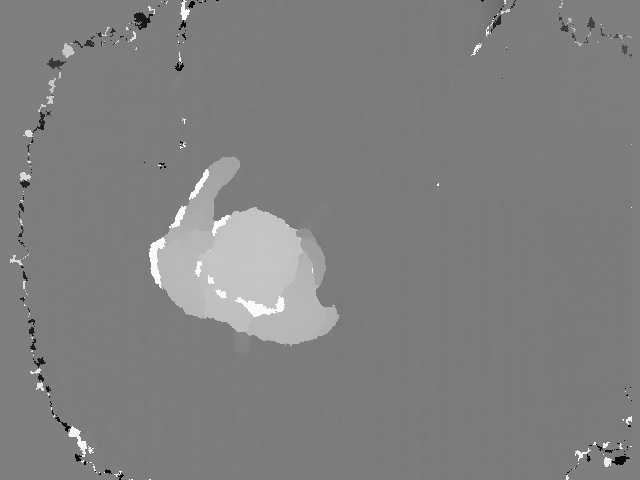
\includegraphics[width=0.5\textwidth]{results/border_effect.png}
  \caption{Border effect is visible as a circle around the scene.}
  \label{fig:border_effect}
\end{figure}

As can be seen in \autoref{fig:border_effect}, this noise is characterized by abrupt variations in depth measure placed very close to each other: it has proven suitable to detect them a first and second order derivative (using Laplace filter) thresholding in the whole image.
Obtained mask was dilated to ensure all artifacts of this noise are removed once applied.

\begin{figure}[htp]
  \centering
  \vspace{-0.5cm}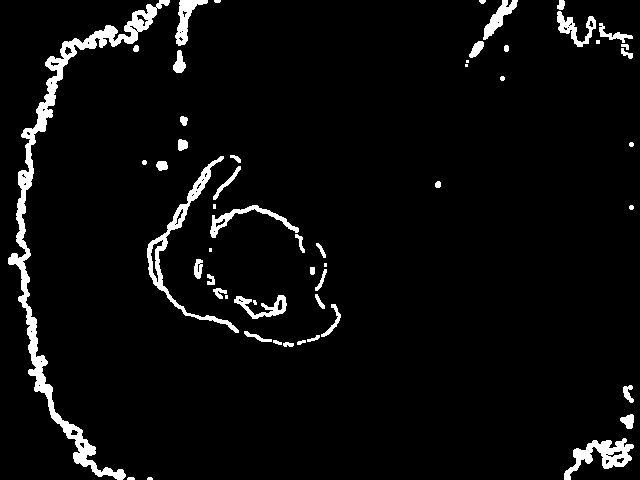
\includegraphics[width=0.5\textwidth]{results/border_mask.png}
  \caption{Mask is applied to depth image where each marked white pixel is replaced by image mean value.}
  \label{fig:border_mask}
\end{figure}

At the end, background is removed from the image revealing only closest points.

\subsection*{People detection}
After the preprocessing phase people shapes can be easily spotted in the image, so a proper algorithm is trained to make this procedure automatic.

Various clustering algorithms were evaluated to split this cloud of points into corresponding people, such as \emph{hierarchical clustering}, but at the end I chose traditional \emph{K-means} clustering.
This decision was taken because of its speed and because it suits the problem very well given its clustering converges towards ellipsoids, very similar to people shapes seen from above.

This approach leads to good results, but unfortunately it requires \emph{a prori} the number of clusters, i.e. the number of people in the scene.

To assess the best value, K-means algorithm was run multiple times and its objective function, \emph{compactness}, was recorded for different values of $K$.

However this metric alone was not suitable to find the optimum, as it is monotonically decreasing in the number of clusters.
A regularization factor was then added in order to prefer simpler configurations where \emph{compactness} decrement in $K$ was getting negligible.

\begin{equation*}
  K^* = \argmin_{K = 1,\, \ldots,\, 6} ~  \log(C_K) - \eta K
\end{equation*}
where $C_K$ is the clustering \emph{compactness}, defined as the sum of square distances of each point to its cluster centroid.

This custom function has similar goals such as \emph{silhouette score}, but it can also evaluate clustering for $K=1$, very relevant in this application.

\section*{Evaluation}
Proposed pipeline works very well in dataset.
Just in one image the number of detected people is wrong (two instead of one), while in the other the count and the position of each individual were properly found.

As a remark, this was achieved only with depth information, while RGB image was only used for final (visual) assessment.

\clearpage
\section*{Appendix}

\foreach \image in {%
  1, 2, 3, 4, 5, 6, 7, 8, 9, 10, 11, 12, 13, 14, 15, 16, 17%
} {%
  \begin{figure}[htp]
    \includegraphics[width=\textwidth]{results/detection-\image .png}
    \caption*{Image number \image}
  \end{figure}
}

\end{document}

%%% Local Variables:
%%% mode: latex
%%% TeX-master: t
%%% End:
